\documentclass[../main.tex]{subfiles}

\begin{document}
\chapter{Gradientenfelder und Differentialformen}\label{chp:gradients}
\section{Gradientenfelder}
Der Stoff dieses Abschnitts ist in den
Abschnitten 181 und 182 in~\cite{heuser} zu finden.

Das motivierende Problem ist folgendermassen zu formulieren.
Sei $U \subset \mathbb{R}^n$ offen und
$X \colon U \to \mathbb{R}^n$ ein stetiges Vektorfeld.
Ist $X$ ein \emph{Gradientenfeld}, das heisst,
existiert
eine differenzierbare Funktion
$f \colon U \to \mathbb{R}^n$,
so dass für alle $p \in U$ gilt, dass ${(\nabla f)}_p = X(p)$?
Dasselbe Problem lässt sich auch in Koordinaten stellen.
Schreibe
\[
  X(p) = \sum_{k=1}^{n} a_k(p) e_k
\]
mit stetigen Komponentenfunktionen $a_k \colon U \to \mathbb{R}$.
Gesucht ist $f \colon U \to \mathbb{R}$ mit
\[
  \frac{\partial f}{\partial x_k} (p) = a_k(p)
\]
für alle
$k \leq n$ und alle $p \in U$.

\begin{specialcase}
  Wir betrachten den Spezialfall $n = 1$.
  Sei $X \colon \mathbb{R} \to \mathbb{R}$ stetig.
  Definiere die Funktion
  $f \colon \mathbb{R} \to \mathbb{R}$ 
  durch 
  \[
    f(p) = \int_{0}^{p} X(t) \, dt.
  \]
  Dann gilt für alle $p \in \mathbb{R}$,
  dass $f'(p) = X(p)$.
  Auf $\mathbb{R}$ sind also alle stetigen Vektorfelder Gradientenfelder.
\end{specialcase}

In Dimension $n \geq 2$ sind nicht alle stetigen
Vektorfelder Gradientenfelder.
Wir werden dazu ein Beispiel konstruieren, indem wir
den Fall $n = 2$ genauer betrachten.
Betrachte ein Vektorfeld $X \colon \mathbb{R}^2 \to \mathbb{R}^2$
mit Komponentenfunktionen $a(x, y)$ und $b(x, y)$.
Sei $f \colon \mathbb{R}^2 \to \mathbb{R}$ differenzierbar
mit $\nabla f = X$.
Falls $b(x, y)$ konstant null ist (insbesondere auch
$\partial f / \partial y = 0)$, dann hängt
$f(x, y)$ nicht von $y$ ab.
Es existiert also eine
differenzierbare Funktion
$g \colon \mathbb{R} \to \mathbb{R}$,
so dass für alle $(x, y) \in \mathbb{R}^2$ gilt,
dass $f(x, y) = g(x)$.
Dann folgt $\partial f / \partial x (x, y) = g'(x)$.
Also hängt $a(x, y) = \partial f / \partial x(x, y) = g'(x)$
nicht von $y$ ab.

\begin{example}
  Das Vektorfeld $X \colon \mathbb{R}^2 \to \mathbb{R}^2$ 
  mit $X(x, y) = (y, 0)$ ist kein Gradientenfeld,
  da $a(x, y) = y$ von $y$ abhängt.
\end{example}

Sei nun $U \subset \mathbb{R}^n$ offen und
\emph{wegzusammenhängend}, das heisst, für
alle $p , q \in U$ existiert eine stetig
differenzierbare
Kurve $\gamma \colon [0, 1] \to U$ mit $\gamma(0) = p$
und $\gamma(1) = q$.
Die Forderung, dass eine stetige Kurve $\gamma$
existiert, impliziert bereits, dass auch eine stetig
differenzierbare Kurve existiert. Wir werden darauf
aber nicht weiter eingehen.

\begin{proposition}\label{prop:gradient-fields-curves}
  Sei $U \subset \mathbb{R}^n$ offen
  und wegzusammenhängend und
  sei $X \colon U \to \mathbb{R}^n$ stetig.
  Dann existiert eine differenzierbare Funktion
  $f \colon U \to \mathbb{R}$ mit $\nabla f = X$,
  genau dann, wenn für alle stetig differenzierbaren
  Wege $\gamma, \overline \gamma \colon [0, 1] \to U$ 
  mit $\gamma(0) = \overline \gamma ( 0) $ und
  $\gamma(1) = \overline\gamma(1)$ gilt, dass
  \[
    \int_{0}^{1} \langle X(\gamma(t)), \dot \gamma(t) \rangle \, dt
    =
    \int_{0}^{1} \langle X(\overline\gamma(t)), 
    \dot{\overline\gamma}(t) \rangle \, dt.
  \]
\end{proposition}

In Worten hängt das Wegintegral von $X$ nur von den Endpunkten
der betrachteten Kurve ab. Äquivalenterweise ist das Integral
von $X$ über alle geschlossenen Wege null.
Geschlossen heisst hier $\gamma(0) = \gamma(1)$.
In diesem Fall gilt für $\overline \gamma(t) = \gamma(0)$ 
dann, dass
\[
  \int_{0}^{1} \langle X(\gamma(t)), \dot \gamma(t) \rangle \, dt
  =
  \int_{0}^{1} \langle X(\overline\gamma(t)), 
  \dot{\overline\gamma}(t) \rangle \, dt = 0.
\]
Umgekehrt seien $\gamma, \overline \gamma \colon [0, 1] \to U$ 
mit $\gamma(0) = \overline \gamma(0)$.
Dann bastle aus $\gamma$ und $\overline \gamma$ 
einen geschlossenen Weg, der zuerst
$\gamma$ durchläuft, und darauf $\overline \gamma$ in umgekehrter
Richtung durchläuft.
Präziser betrachten wir den Weg
\begin{align*}
  \gamma \cup - \overline \gamma \colon [0, 1] & \to U \\
  t & \mapsto 
  \begin{cases}
    \gamma(2t) & t \leq 1/2,\\
    \overline \gamma (2 - 2t) & t \geq 1/2.
  \end{cases}
\end{align*}


\begin{proof}[Beweis von Proposition~\ref{prop:gradient-fields-curves}]
  Sei $f \colon U \to \mathbb{R}$ differenzierbar
  mit $\nabla f = X$.
  Sei weiterhin $\gamma \colon [0, 1] \to U$ stetig differenzierbar.
  Für die Komposition $f \circ \gamma \colon [0, 1] \to \mathbb{R}$ 
  gilt dann für alle $t \in (0, 1)$, dass
  \[
    \frac{d}{dt}(f \circ \gamma) (t)
    = {(Df)}_{\gamma(t)}({(D\gamma)}_t(1))
    = \langle {(\nabla f)}_{\gamma(t)}, \dot \gamma(t) \rangle.
  \]
  Wir folgern mit Hilfe der stetigen Differenzierbarkeit
  von $\gamma$, dass
  \begin{align*}
    \int_{0}^{1} \langle X(\gamma(t)), \dot \gamma(t) \rangle \, dt
    &= \int_{0}^{1} \langle {(\nabla f)}_{\gamma(t)}, 
    \dot \gamma(t) \rangle \, dt \\
    &= \int_{0}^{1} \frac{d}{dt} (f \circ \gamma)(t) \, dt  \\
    &= f(\gamma(1)) - f(\gamma(0)).
  \end{align*}
  Insbesondere ist, falls $\gamma(1) = \gamma(0)$ gilt, das Wegintegral
  von $X$ null.

  Sei nun umgekehrt $X \colon U \to \mathbb{R}^n$
  ein stetig differenzierbares Vektorfeld, dessen geschlossenen
  Wegintegrale alle verschwinden.
  Wir konstruieren eine \emph{Potentialfunktion}
  $f \colon U \to \mathbb{R}$ mit $\nabla f = X$.
  Sei $p \in U $ fest gewählt.
  Sei $q \in U$.
  Wähle $\gamma \colon [0, 1] \to U$ stetig differenzierbar
  mit $\gamma(0) = p$ und $\gamma(1) = q$.
  Setze
   \[
     f(q) = \int_{0}^{1} \langle X(\gamma(t)), \dot \gamma(t) \rangle \, dt.
  \]
  Wir bemerken, dass $f(q)$ nicht von der Wahl von $\gamma$ abhängt.
  Wir zeigen nun, dass für alle $q \in U$ gilt,
  dass ${(\nabla f)}_q = X(q)$.
  Sei dazu $h \in \mathbb{R}^n$ beliebig.
  Für kleine $t \in \mathbb{R}$ gilt dann, dass $q + th$
  auch noch in $U$ liegt (denn $U$ ist offen).
  Wir haben
  \[
    \langle {(\nabla f)}_q, h \rangle
    = {(Df)}_q(h) = \lim_{t \to 0} \frac{f(q + th) - f(q)}{t}.
  \]
  Betrachte den Weg  
  \begin{align*}
    \delta \colon [0, t] & \to U \\
    s & \mapsto q + sh.
  \end{align*}
  Es existiert $t > 0$ so, dass $\delta([0, t]) \subset U$.
  Nach Konstruktion gilt
  \begin{align*}
     f(q + th) - f(q) 
     &=\int_{0}^{t} \langle X(\delta(s)), \dot \delta(s) \rangle \, ds  \\
     &= \int_{0}^{t} \langle X(q + sh), h \rangle \, ds \\
     &= \int_{0}^{t} \langle X(q), h \rangle \, ds
     + \int_{0}^{t} \langle X(q + sh) - X(q), h \rangle \, ds \\
     &= t \langle X(q), h \rangle + R
  \end{align*}
  für
  \[
    R = \int_{0}^{t} \langle X(q + sh) - X(q), h \rangle \, ds.
  \]
  Schätze ab, dass
  \[
    |R| \leq t \cdot \Vert X (q + sh) - X(q) \Vert_2 \cdot \Vert h \Vert_2.
  \]
  Es gilt also
  \[
    \lim_{t \to 0} \frac{|R|}{t} = 0,
  \]
  da $X$ stetig an der Stelle $q$ ist.
  Daraus folgt, dass
  \[
    {(Df)}_q (h) = \lim_{t \to 0} \frac{f(q + th) - f(q)}{t}
    = \langle X(q), h \rangle,
  \]
  was ${(\nabla f)}_q = X(q)$ impliziert.
\end{proof}

\begin{example}
  Sei
  \begin{align*}
    X \colon \mathbb{R}^2 & \to \mathbb{R}^2 \\
    (x, y) & \mapsto (-y, x)
  \end{align*}
  eine Rotation um den Winkel $\pi/2$.
  Betrachte den Weg
  \begin{align*}
    \gamma \colon [0, 1] & \to \mathbb{R}^2 \\
    t & \mapsto (\cos(2 \pi t), \sin(2 \pi t)).
  \end{align*}
  Es gilt $\gamma(0) = \gamma(1) = (1, 0)$.
  Berechne aber
  \[
    \int_{0}^{1} \langle X(\gamma(t)), \dot \gamma(t) \rangle \, dt
    = 2\pi \cdot \int_{0}^{1} \cos^2(2 \pi t) + \sin^2(2 \pi t) \, dt
    = 2 \pi \neq 0.
  \]
  Somit ist $X$ kein Gradientenfeld.
\end{example}

\subsection*{Lemma von Poincaré}

Leider ist die Bedingung, dass alle geschlossenen Wegintegrale
null sind, impraktikabel.
Die Bedingung kann nämlich nur schwer dazu verwendet werden,
zu verifizieren, dass eine gegebenes Vektorfeld $X$ 
ein Gradientenfeld ist.
Das Lemma von Poincaré unten liefert ein leichter überprüfbares
Kriterium

Sei $U \subset \mathbb{R}^n$ offen
und $X \colon U \to \mathbb{R}^n$ differenzierbar.
Falls eine differenzierbare Funktion
$f \colon U \to \mathbb{R}$ mit $\nabla f = X$ existiert,
dann ist $f$ automatisch zweimal differenzierbar
(da $\nabla f = X \colon U \to \mathbb{R}^n$ differenzierbar ist).
Nach dem Satz von Schwarz gilt für alle
$i, j \in \{1, \dots, n\}$ und alle $p \in U$, dass
\[
  \frac{\partial^2 f}{\partial x_j \partial x_i}(p) =
  \frac{\partial^2 f}{\partial x_i \partial x_j}(p).
\]
Schreibe nun
\[
  X(p) = \sum_{k=1}^{n} a_k(p) e_k
\]
mit differenzierbaren Komponentenfunktionen $a_k \colon U \to \mathbb{R}$.
Aus $\nabla f = X$ folgen nun die ``Poincaré-Bedingungen''
\[
  \frac{\partial a_i}{\partial x_j}(p) = \frac{\partial a_j}{\partial x_i}(p).
\]

Wir betrachten nun den Spezialfall $n = 3$.
Sei $X \colon \mathbb{R}^3 \to \mathbb{R}^3$ 
differenzierbar mit Komponenten $a, b, c \colon \mathbb{R}^3 \to \mathbb{R}$.
Dann sind die Poincaré-Bedingungen äquivalent zu den Gleichungen
\begin{align*}
  \frac{\partial a}{\partial y} &= \frac{\partial b}{\partial x}, \\
  \frac{\partial a}{\partial z} &= \frac{\partial c}{\partial x}, \\
  \frac{\partial b}{\partial z} &= \frac{\partial c}{\partial y}.
\end{align*}

\begin{definition}
  Sei $X \colon \mathbb{R}^3 \to \mathbb{R}^3$ differenzierbar
  mit Komponenten $a, b, c$.
  Dann ist die \emph{Rotation} von $X$ gegeben durch
  \[
    \text{rot}(X) =
    \begin{pmatrix}
      {\partial b}/{\partial z} - {\partial c}/{\partial y} \\
      {\partial c}/{\partial x} - {\partial a}/{\partial z} \\
      {\partial a}/{\partial y} - {\partial b}/{\partial x}.
    \end{pmatrix}
  \]
\end{definition}

Es folgt direkt, dass die Poincaré-Bedingungen für
ein differenzierbares Vektorfeld $X$ äquivalent
zur Forderung $\text{rot}(X) = 0$ sind.
Leider reichen die Poincaré-Bedingungen im allgemeinen
nicht aus, um ein Vektorfeld $X$ als Gradientenfeld
zu charakterisieren.

\begin{example}
  Sei $U = \mathbb{R}^2 \setminus \{0\}$.
  Sei  
  \begin{align*}
    X \colon \mathbb{R}^2 \setminus \{0\} & \to \mathbb{R}^2 \\
    (x, y) & \mapsto (-y/(x^2 + y^2), x/(x^2 + y^2)).
  \end{align*}
  Es gilt für alle $x, y \neq (0, 0)$, dass
  $\partial a / \partial y (x, y) = \partial b/ \partial x(x, y)$,
  vergleiche Serie 10.
  Wir bemerken aber, dass die Einschränkung von $X$ 
  auf $S^1 = \left\{(x, y) \in \mathbb{R}^2 \mid x^2 + y^2 = 1\right\}$ 
  mit dem Vektorfeld $\overline X(x, y) = (-y, x)$ übereinstimmt.
  Vom Vektorfeld $\overline X$ wissen wir aus einem Beispiel
  oben aber bereits, dass es ein geschlossenes nicht-verschwindendes
  Wegintegral zulässt.
  Konkreter gilt für den Weg
  $\gamma(t) = (\cos(2 \pi t), \sin (2 \pi t))$, dass
  \[
    \int_{0}^{1} \langle X(\gamma(t)), \dot \gamma(t) \rangle \, dt
    = 2\pi,
  \]
  also ist $X$ kein Gradientenfeld.
\end{example}

\begin{definition}
  Eine Teilmenge $U \subset \mathbb{R}^n$ 
  heisst \emph{sternförmig} bezüglich einem Punkt $p \in U$,
  falls für alle $q \in U$ und alle $t \in [0, 1]$ 
  gilt, dass $p + t(q - p) \in U$.
  In anderen Worten liegt der Geradenabschnitt zwischen $p$ und $q$ 
  noch vollständig in $U$.
\end{definition}

\begin{examples}
  \leavevmode
  \begin{enumerate}[(1)]
    \item Die Menge $U = \mathbb{R}^2 \setminus \{0 \}$ ist bezüglich
      keinem Punkt sternförmig.
      Tatsächlich geht die Strecke zwischen 
      $p \in \mathbb{R}^2 \setminus \{0\}$
      und $-p$ durch den Nullpunkt, welcher nicht in $U$ liegt.
    \item Die Menge $\mathbb{R}^2 \setminus (\mathbb{R}_{\leq 0}
      \times \{0\})$ (die Ebene ohne die negative $x$-Achse) 
      ist sternförmig bezüglich dem Punkt 
      $p = (1, 0)$.
    \item Alle konvexen Teilmengen von $\mathbb{R}^n$ sind sternförmig.
  \end{enumerate}
\end{examples}

\begin{theorem}[Poincaré Lemma, ca. 1900]
  Sei $U \subset \mathbb{R}^n$ offen und sternförmig bezüglich
  $p \in U$. Sei weiterhin $X \colon U \to \mathbb{R}^n$ 
  differenzierbar, so dass die Poincaré-Bedingungen
  auf $U$ erfüllt sind.
  Dann existiert eine differenzierbare Funktion
  $f \colon U \to \mathbb{R}$ mit $\nabla f = X$.
\end{theorem}

\begin{proof}
  Um die Notation zu vereinfachen werden wir $p = 0$ annehmen.
  Sei $q \in U$.
  Schreibe $X = a_1 e_1 + \cdots + a_n e_n$ und
  $q = x_1 e_1 + \cdots x_n e_n$.
  Definiere
  \begin{align*}
    \gamma \colon [0, 1] & \to U \\
    t & \mapsto tq
  \end{align*}
  und
  \[
    f(q) = \int_{0}^{1} \langle X(\gamma(t)),
    \dot \gamma (t) \rangle \, dt.
  \]
  Berechne
  \begin{align*}
    f(q)
    & = \int_{0}^{1} \langle X(tq), q \rangle \, dt\\
    &= \int_{0}^{1} \sum_{i=1}^{n} a_i(tx_1, \dots, tx_n) \cdot x_i \, dt.
  \end{align*}
  Sei $k \leq n$ und berechne mit Hilfe vom Lemma unten, dass
  \begin{align*}
    \frac{\partial f}{\partial x_k}(q)
    & = \frac{\partial f}{\partial x_k } (x_1, \dots, x_n)\\
    &= \frac{\partial}{\partial x_k} \int_{0}^{1} 
    \sum_{i=1}^{n} a_i (tq) \cdot x_i \, dt \\
    &= \int_{0}^{1} \frac{\partial}{\partial x_k}
    \sum_{i=1}^{n} a_i(tq) \cdot x_i \, dt.
  \end{align*}
  Es gilt
  \begin{align*}
    \frac{\partial}{\partial x_k}
    \sum_{i=1}^{n} a_i(tq) \cdot x_i
    &= \sum_{i=1}^{n} \frac{\partial a_i}{\partial x_k}
    (tx_1, \dots, tx_n) \cdot t \cdot x_i
    + \sum_{i=1}^{n} a_i(tq) \cdot \frac{\partial a_i}{\partial x_k}\\
    &= \sum_{i=1}^{n} \left( \frac{\partial a_i}{\partial x_k}
    (tx_1, \dots, tx_n) \cdot t \cdot x_i \right)
    + a_k(tq) \\
    &= \frac{d}{dt} (t \cdot a_k(tx_1, \dots, tx_n)).
  \end{align*}
  Tatsächlich ist nämlich
  \begin{align*}
    \frac{d}{dt}(t \cdot a_k(tx_1, \dots, tx_n))
    & = a_k(tq) + \sum_{i=1}^{n} t \cdot \frac{\partial a_k}{\partial x_i}
    (tx_1, \dots, tx_n) \cdot x_i,
  \end{align*}
  also erhalten wir mit Hilfe der Poincaré-Bedingungen
  die gewünschte Gleichheit.
  Es folgt, dass
  \begin{align*}
    \frac{\partial f}{\partial x_k}(q)
    & = \int_{0}^{1} \frac{d}{dt}(t a_k (tq)) \, dt\\
    &= a_k(q),
  \end{align*}
  also gilt $\nabla f = X$.
\end{proof}

\begin{lemma*}
  Sei $g \colon {[0, 1]}^2 \to \mathbb{R}$ stetig differenzierbar.
  Dann gilt für alle $x \in (0, 1)$, dass
  \[
    \frac{\partial}{\partial x} \int_{0}^{1} g(x, y) \, dy
    = \int_{0}^{1} \frac{\partial}{\partial x} g(x, y) \, dy.
  \]
\end{lemma*}

\begin{proof}
  Berechne
  \begin{align*}
    \frac{\partial}{\partial x}
    \int_{0}^{1} g(x, y) \, dy
    &= \lim_{h \to 0} \frac{1}{h}
    \int_{0}^{1} g(x + h, y) - g(x, y) \, dy.
  \end{align*}
  Nach dem Mittelwertsatz existiert
  $\overline x \in [x, x + h]$ mit
  \[
    \frac{g(x + h, y) - g(x, y)}{h}= \frac{\partial}{\partial x}
    g(\overline x, y).
  \]
  Sei nun $\varepsilon > 0$.
  Da $\partial g / \partial x \colon {[0, 1]}^2 \to \mathbb{R}$ 
  stetig ist, und weiterhin ${[0, 1]}^2$ kompakt,
  ist $\partial g/\partial x$ sogar gleichmässig stetig
  auf  ${[0, 1]}^2$.
  Also existiert $\delta > 0$ so, dass für alle
  $x, \overline x, y \in [0,1]$ mit $|x - \overline x| \leq \delta$ 
  gilt, dass
  \[
    \left| \frac{\partial g}{\partial x}(\overline x, y)
    - \frac{\partial g}{\partial x}(x, y) \right| \leq \varepsilon.
  \]
  Für $h \in \mathbb{R}$ mit $|h| \leq \delta$ 
  gilt also (da $\overline x \in [x, x + h])$, dass
  \begin{align*}
    \left| \int_{0}^{1} \frac{1}{h}
    g(x + h, y) - g(x, y)\, dy
    - \int_{0}^{1} \frac{\partial}{\partial x}g(x, y) \, dy \right|
    &= \left| 
    \int_{0}^{1} 
    \frac{\partial}{\partial x} g(\overline x, y)
    - \frac{\partial}{\partial x}g(x, y)\, dy \right| 
    \leq \varepsilon.
  \end{align*}
  Daraus folgt, dass wir den Grenzwert mit dem Integral
  vertauschen können.
\end{proof}

\begin{remark}
  Die Annahme, dass $U$ sternförmig ist, wird im Beweis
  verwendet um ``kanonische'' Wege zu wählen.
  Lässt man die Bedingung der Sternförmigkeit weg,
  lässt sich $f$ nicht eindeutig definieren.

  Tatsächlich geht das bei Gebieten mit ``Löchern''
  schief. Betrachte zum
  Beispiel das Vektorfeld
  \begin{align*}
    X \colon \mathbb{R}^2 \setminus \{0\} & \to \mathbb{R}^2\\
    (x, y) & \mapsto (-y/(x^2 + y^2), x/(x^2 + y^2)),
  \end{align*}
  welches die Poincaré-Bedingungen erfüllt, aber dennoch
  kein Gradientenfeld ist (da das Wegintegral um den Einheitskreis
  nicht verschwindet).
\end{remark}

\begin{proposition}\label{prop:low-dimensions}
  \leavevmode
  \begin{enumerate}[\normalfont(i)]
    \item Sei $X = (a, b) \colon \mathbb{R}^2 \setminus \{0\} \to \mathbb{R}^2$ 
      differenzierbar. Dann ist $X$ ein Gradientenfeld, genau dann wenn
      die Poincaré-Bedingung
      $\partial b / \partial x = \partial a / \partial y$ 
      erfüllt ist, und gleichzeitig
      \[
        \int_{0}^{1} \langle X(\gamma(t)), \dot \gamma(t) \rangle \, dt = 0
      \]
      für den Weg $\gamma(t) = (\cos(2\pi t), \sin(2 \pi t))$ gilt.
    \item Sei 
      $X \colon \mathbb{R}^3 \setminus \{0\} \to \mathbb{R}^3$ 
      differenzierbar.
      Dann ist $X$ ein Gradientenfeld, genau dann, wenn $\textup{rot}(X) = 0$
      gilt (und keine Zusatzbedingung).
  \end{enumerate}
\end{proposition}

\begin{proof}
  Die beiden Hinrichtungen ($\Rightarrow$) haben wir bereits behandelt.
  Die Rückrichtungen ($\Leftarrow$) beweisen wir einzeln.
  \begin{enumerate}[(i)]
    \item Sei $X = (a, b) \colon \mathbb{R}^2 \setminus \{0\} \to \mathbb{R}^2$ 
      ein differenzierbares Vektorfeld mit $\partial b / \partial x =
      \partial a / \partial y$.
      Schreibe $U = \mathbb{R}^2 \setminus \{0\} = U_N \cup U_S$, wobei
      \begin{align*}
        U_N & = \mathbb{R}^2 \setminus \left\{(0, y) \mid y \leq 0\right\}, \\
        U_S & = \mathbb{R}^2  \setminus \left\{(0, y) \mid y \geq 0 \right\}.
      \end{align*}
      Die beiden Mengen $U_N$ und $U_S$ sind offen und sternförmig.
      Nach dem Poincaré Lemma existieren 
      differenzierbare Funktionen $f_N \colon U_N \to \mathbb{R}$ 
      sowie $f_S \colon U_S \to \mathbb{R}$ mit
      $\nabla f_N = X|_{U_N}$ und $\nabla f_S = X|_{U_S}$.
      Wir können
      durch Addition einer Konstante 
      $f_N$ und $f_S$ so wählen, dass
      $f_N(e_1) = f_S(e_1)$.

      Wir zeigen nun, dass für alle $q \in U_S \cap U_N$ gilt,
      dass $f_N(q) = f_S(q)$.
      Schreibe dazu $U_S \cap U_N = U_L \cup U_R$ mit
      \begin{align*}
        U_L & = \left\{(x, y) \in \mathbb{R}^2 \mid x < 0 \right\}, \\
        U_R &= \left\{(x, y) \in \mathbb{R}^2 \mid x > 0\right\}.
      \end{align*}
      Da $f_N(e_1) = f_S(e_1)$ und $\nabla f_N = X = \nabla f_S$ 
      auf $U_R$ gilt, folgt für alle $q \in U_R$, dass
      $f_N(q) = f_S(q)$.
      Dies liegt daran, dass $U_R$ wegzusammenhängend ist,
      und dass eine Stammfunktion einer differenzierbaren Funktion
      aus einem Funktionswert (in unserem Fall $e_1$)
      und dem Wegintegral rekonstruiert werden kann.

      Zu zeigen bleibt, dass $f_N = f_S$ auf $U_L$ gilt.
      Mit demselben Argument wie oben reicht es zu zeigen,
      dass $f_N(-e_1) = f_S(-e_1)$ gilt.
      % Dazu bemerken wir, dass
      % \[
      %   \int_{0}^{1/2} \langle X(\gamma(t)), \dot \gamma(t) \rangle \, dt
      %   +
      %   \int_{1/2}^{1} \langle X(\gamma(t)), \dot \gamma(t) \rangle \, dt
      %   = 0.
      % \]
      Schreibe dazu
      \[
        A = 
        \int_{0}^{1/2} \langle X(\gamma(t)), \dot \gamma(t) \rangle \, dt
      \]
      und
      \[
        B = 
        \int_{1/2}^{1} \langle X(\gamma(t)), \dot \gamma(t) \rangle \, dt.
      \]
      Berechne, dass
      \(
        A = f_N(-e_1) - f_N(e_1)
      \)
      (da auf $U_N$ gilt,
      dass $X = \nabla f_N$),
      und $B = f_S(e_1) - f_S(-e_1)$
      (da auf $U_S$ gilt, dass $X = 
      \nabla f_S$),
      siehe Abbildung~\ref{fig:e1tominuse1}.
      Übrig bleibt, dass
      $f_N(-e_1) = f_S(-e_1)$ gilt.

      \begin{figure}[htb] 
        \centering
        \begin{minipage}{0.30\textwidth}
          \centering
          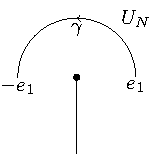
\includegraphics{figures/e1tominuse1}
        \end{minipage}%
        \begin{minipage}{0.30\textwidth}
          \centering
          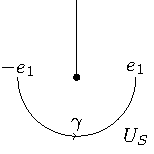
\includegraphics{figures/minuse1toe1}
        \end{minipage}%
        \caption{Der Grund, dass $f_N(-e_1) = 
        f_S(-e_1)$ gilt}%
        \label{fig:e1tominuse1}
      \end{figure}

      Definiere nun
      \begin{align*}
        f \colon \mathbb{R}^2 \setminus \{0\} & \to \mathbb{R} \\
        q & \mapsto 
        \begin{cases}
          f_N(q) & q \in U_N, \\
          f_S(q) & q \in U_S.
        \end{cases}
      \end{align*}
      Dank der oberen Betrachtungen
      ist $f$ wohldefiniert.
      Weiter gilt für alle
      $q \in \mathbb{R}^2$, dass
      $\nabla f = X$.

    \item Sei
      $X \colon \mathbb{R}^3 \setminus \{0\}
      \to \mathbb{R}^3$ 
      differenzierbar mit $\text{rot}(X) = 0$.
      Schreibe
      $\mathbb{R}^3 \setminus \{0\}
      = U_N \cup U_S$ 
      mit
      \begin{align*}
        U_N & = \mathbb{R}^3 \setminus
        \left\{(0, 0, z) \mid z \leq 0\right\},\\
        U_S & = \mathbb{R}^3 \setminus
        \left\{(0, 0, z) \mid z \leq 0\right\}.
      \end{align*}
      Nach dem Poincaré Lemma existieren differenzierbare Funktionen
      $f_N \colon U_N \to \mathbb{R}$ 
      und $f_S \colon U_S \to \mathbb{R}$ mit
      $\nabla f_N = X|_{U_N}$ und $\nabla f_S = X|_{U_S}$.
      Wiederum können wir
      $f_N(e_1) = f_S(e_1)$ einrichten.
      Dann gilt für alle
      $q \in U_N \cap U_S$, dass
      $f_N = f_S(q)$.
      Tatsächlich ist $U_N \cap U_S = \mathbb{R}^3
      \setminus \left\{(0, 0, z) \mid z \in \mathbb{R}\right\}$ 
      wegzusammenhängend.
      Via Wegintegral folgt also $f_N = f_S$ auf ganz $U_N \cap U_S$.
      Definiere dann $f$ wie oben. \qedhere
  \end{enumerate}
\end{proof}

\begin{exercise}
  Zeige die Konklusion von Punkt (ii) in Proposition~\ref{prop:low-dimensions}
  für $\mathbb{R}^3 \setminus F$, wobei $F \subset \mathbb{R}^3$ 
  eine endliche Menge ist.
\end{exercise}

\section{Differentialformen}
Sei $U \subset \mathbb{R}^n$ offen.
Eine \emph{$1$-Form} auf $U$ ist eine stetige Abbildung
$\omega \colon U \to {(\mathbb{R}^n)}^*$.
Hier ist ${(\mathbb{R}^n)}^*$ der \emph{Dualraum} von $\mathbb{R}^n$.
Er besteht aus allen linearen Abbildungen 
$L \colon \mathbb{R}^n \to \mathbb{R}$.
Die Elemente $e_k^* \colon \mathbb{R}^n \to \mathbb{R}$ 
welche durch die Forderung
\[
  e_k^*(e_i) =
  \begin{cases}
    1 & i = k, \\
    0 & i \neq k
  \end{cases}
\]
eindeutig definiert sind, bilden eine Basis von
${(\mathbb{R}^n)}^*$.
Deren Elemente werden häufig mit $x_k = e_k^*$ 
bezeichnet und heissen \emph{Koordinatenabbildungen}.

Sei nun $f \colon U \to \mathbb{R}$
stetig differenzierbar.
Für alle $p \in U$ erhalten wir dann das Differential
${(Df)}_p \in {(\mathbb{R}^n)}^*$.
Die \emph{totale Ableitung} von $f$ ist die $1$-Form
\begin{align*}
  df \colon U & \to {(\mathbb{R}^n)}^* \\
  p & \mapsto {(Df)}_p.
\end{align*}
Für alle $i \in \{1, \dots, n\}$ gilt
${(Df)}_p(e_i) = \partial f / \partial x_i (p)$.
Die Abbildungsmatrix von ${(Df)}_p$ ist somit ein Zeilenvektor mit
Einträgen $\partial f/ \partial x_i (p)$.
Somit können wir schreiben, dass
\[
  {(Df)}_p =
  \sum_{i=1}^{n} \frac{\partial f}{\partial x_i}(p) \cdot e_i^*.
\]

Sei $k \in \{1, \dots, n\}$.
Für $x_k \colon \mathbb{R}^n \to \mathbb{R}$ gilt
für alle $p \in \mathbb{R}^n$, dass
${(Dx_k)}_p = x_k$, da $x_k$ linear ist.
Also ist $dx_k \colon \mathbb{R}^n \to \mathbb{R}$ 
gegeben durch $dx_k(p) = x_k$, da $x_k$ linear ist.
Somit ist $dx_k$ eine konstante $1$-Form,
beziehungsweise ein konstantes Feld von linearen Abbildungen.
Für allgemeinere $f \colon U \to \mathbb{R}$
erhalten wir
\[
  df = \sum_{i=1}^{n} \frac{\partial f}{\partial x_i} dx_i.
\]

Sei $\omega \colon U \to {(\mathbb{R}^n)}^*$ eine beliebige $1$-Form,
welche einen Punkt $p$ auf eine lineare Funktion $\omega_p
\in {(\mathbb{R}^n)}^*$ sendet.
Für $k \in \{1, \dots, n\}$ definiere
\begin{align*}
  a_k \colon U & \to \mathbb{R} \\
  p & \mapsto \omega_p(e_k)
\end{align*}
Wir erhalten somit
\[
  \omega = \sum_{i=1}^{n} a_i dx_i.
\]
Die Abbildung $\omega_p$ ist die lineare Abbildung
mit Abbildungsmatrix $(a_1(p), \dots, a_n(p))$.
Wir nennen  $\omega \colon U \to {(\mathbb{R}^n)}^*$ 
\emph{differenzierbar}, falls alle
$a_k \colon U \to \mathbb{R}$ differenzierbar sind.

\begin{question}
  Sei $\omega \colon U \to {(\mathbb{R}^n)}^*$ eine
  differenzierbare $1$-Form.
  Existiert dann $f \colon U \to \mathbb{R}$ mit
  $df = \omega$?
\end{question}

In Komponenten ist das äquivalent zu der Forderung,
dass
$\partial f / \partial x_i = a_i$
gilt.
Dieses Problem haben wir für sternförmige
$U \subset \mathbb{R}^n$ bereits gelöst:
eine positive Antwort zur Frage ist äquivalent zu
den Poincaré-Bedingungen.

\begin{definition}
  Sei $\gamma \colon [0, 1] \to U$ stetig differenzierbar.
  Das \emph{Wegintegral} von $\omega$ entlang $\gamma$ ist
  \[
    \int_\gamma \omega = \int_{0}^{1} \omega_{\gamma(t)}(\dot \gamma(t)) \, dt.
  \]
\end{definition}

\begin{remark}
  Im Spezialfall $\omega = df$ gilt
  \[
    \int_\gamma df = \int_{0}^{1} df_{\gamma(t)}(\dot \gamma(t)) \, dt
    = \int_{0}^{1} {(Df)}_{\gamma(t)}(\dot \gamma(t)) \, dt
    = f(\gamma(1)) - f(\gamma(0)).
  \]
  Falls $\gamma$ geschlossen ist, dann gilt
  $\int_\gamma df = 0$.
\end{remark}

\begin{definition}
  Sei $\omega \colon U \to {(\mathbb{R}^n)}^*$ differenzierbar.
  seien weiterhin $p \in U$ und $v, w \in \mathbb{R}^n$.
  Die \emph{äussere Ableitung} von $\omega$ ist
  \[
    {(d\omega)}_p(v, w)
    = \lim_{s \to 0} \frac{1}{s^2} \int_{\gamma_s} \omega,
  \]
  wobei $\gamma_s$ der stückweise affine 
  geschlossene Weg zwischen den
  Punkten $p, p+s, p+ s(v + w), p+sw$ ist.
  Diese Punkte sind die Eckpunkte eines Parallelogramms.
\end{definition}

Die Abbildung ${(d \omega)}_p$ ist ein Spezialfall einer sogenannten
2-Form. Im Falle von $\omega = df$ wissen wir,
da Wegintegrale auf geschlossenen Kurven verschwinden,
dass das Resultat relativ unspektakulär ist.

\begin{theorem*}
  Sei $f \colon U \to \mathbb{R}$ zwei Mal
  differenzierbar.
  Dann gilt $ddf = 0$.
\end{theorem*}

Differentialformen sind sowohl in der Physik (häufig als Tensoren)
und in der Homologietheorie anzutreffen.
In der Homologietheorie (konkreter, der De Rham Kohomologietheorie)
ist deren Nutzen, dass sie in höherdimensionalen Räumen
Löcher erkennen können. Hier sind nämlich Vektorfelder gescheitert:
In $\mathbb{R}^3 \setminus \{0\}$ existiert kein Vektorfeld,
welches die Poincaré-Bedingungen erfüllt, aber 
nicht ein Gradientenfeld ist.
Es existiert aber sehr wohl eine $2$-Form auf
$\mathbb{R}^3 \setminus \{0\}$, welche nicht von der Form
$d \omega$ für eine $1$-Form $\omega$ ist.

\end{document}

